\documentclass[a4paper, 12pt, headsepline]{scrartcl}
    % General document formatting
    %\usepackage[margin=0.7in]{geometry}
    %\usepackage[parfill]{parskip}
    \usepackage[utf8]{inputenc}
    %\usepackage[headsepline,footsepline]{scrpage2}
    \usepackage[onehalfspacing]{setspace}
    \usepackage{times}
    \usepackage{graphicx}
    \graphicspath{ {images/} }


% Header and Footer Formatting-----------------------------------------------------------------------
%   Formatting of Header and Footer
% ---------------------------------------------------------------------------------------------------
%\pagestyle{scrheadings}
%\clearscrheadfoot
%\ohead{\headmark}
%\ofoot{\pagemark}

% Title Page Information-----------------------------------------------------------------------------
%   These are the informations printed on the title page of the article
% ---------------------------------------------------------------------------------------------------

\title{Project trckr}
\subtitle{Technical Article}
\date{May 2018}
\author{
Ankeshian, Gabriel\\
\texttt{ankesgab@students.zhaw.ch}
\and
Balidis, Dimitri\\
\texttt{baliddim@students.zhaw.ch}
\and
Christen, Luca\\
\texttt{chrisluc@students.zhaw.ch}
\and
Jossi, Savino\\
\texttt{jossisav@students.zhaw.ch}
\and
Milenkovic, Daniel\\
\texttt{milendan@students.zhaw.ch}
\and
Nominato, Angelica Helena Moreira Alves\\
\texttt{moreiane@students.zhaw.ch}
\and
Pacassi, David\\
\texttt{pacasdav@students.zhaw.ch}}

\begin{document}
\maketitle
\pagebreak

% Abstract-----------------------------------------------------------------------------
%   This is the abstract of the technical article
% -------------------------------------------------------------------------------------
\begin{abstract}
The main goal of the present article is to describe the idea, goals and main functionalities of the web based app trckr. Trckr is for everyone,
who works on a project and wants an intuitive and simple web tool with easy to learn handling.\\
To have an easy development, the backend is written in Python with the help of the framework Django, the frontend with the Javascript
framework Vue.js. Users are able to create and edit projects after a successful registration. Time tracking starts with single tasks
a user creates.\\
In order to compete with other tools and web services, trckr has big advantages in performance and usability. To extend the reach of trckr, more
functions are planned to display projects and tasks in a user-friendly manner. These planned features will give trckr a great advantage towards ever
increasing complexity in project management and task tracking, this would be especially useful for larger companies. Additionally we provide trckr
as an open source solution and everybody can contribute features that could be useful for the greater user base.

\end{abstract}

\pagebreak

% Table of Contents-----------------------------------------------------------------------------
%   This is the table of contents
% -------------------------------------------------------------------------------------------

\tableofcontents

\pagebreak

% Introduction-----------------------------------------------------------------------------
%   This is the information printed on the title page of the article
% ------------------------------------------------------------------------------------------
\section{Introduction}
Time tracking is an important process for daily business to have insight on the productivity of a team, this lead to ever improving processes and tools
that allow for easier time tracking, no matter which branch. This also lead to multiple methods and tools being developed and enhanced in parallel,
many methods are not very helpful for a certain branch because they might give enough insight or have too many features that are not going to be used.
Yet these methods might be good for another branch, this tells us, that diversity is in no way an issue and tools and methods are adapting to teams,
and not the other way around.

\subsection{Objectives}
The goal with project trckr is to develop and distribute a time tracking webapp, that is very easy to understand and use. It is highly important to
have the least amount of steps possible, for a user to track his time on single tasks.

\subsection{Main Features}
The user is able to:
\begin{itemize}
    \item register and login to trckr
    \item create and edit projects
    \item create, track and edit tasks
    \item visit trckr also on a mobile browser
\end{itemize}


\section{Technolgies}


\subsection{Django}
Django is an open source web framework written in Python. It is very useful for fast, clean and simple development of web applications.\\
One of the main advantages is its fast setup, therefore you can start developing your application very quick through it's Model-View-Presenter scheme.
Django comes with support of various database integrations. Many users compare Django with Ruby On Rails, but written in Python.
Django follows also the DRY principle (Don't Repeat Yourself).

\subsection{PostgreSQL}
Trckr runs with a PostgreSQL database in the backend. PostgreSQL is fully supported by Django and
implemented from the beginning. With Django in use, not much has to be configured for the database, because
the whole database is written by Django.

\subsection{Vue.js}
Vue.js is a progressive framework for building user interfaces.\cite{vuejs} Trckr is developed with Vue.js mainly for its simplicity and the rather shallow learning curve it provides to unexperienced developers.
The features that Vue.js provides, allow the creation of data structures that can easily be displayed in the HTML of a page. This and the ability to easily make calls to the backend makes it a perfect all-round framework for trckr.


% Results-----------------------------------------------------------------------------
%   This is the information printed on the title page of the article
% -------------------------------------------------------------------------------------------
\section{Results}
As you can see in the figure \ref{fig:architecture}, we have built a pretty simple architecture,
including Django with PostgreSQL in the backend and a frontend based on Node.

\begin{figure}[h]
    \includegraphics[width=8cm]{architecture}
    \caption{Architecture of trckr}
    \label{fig:architecture}
\end{figure}

\subsection{API}
The backend of the trckr application implements a RESTful API using the Django
REST framework. The API provides basic CRUD operations for all the entities
available in the database. There are five main endpoints to retrieve and save
data on the server: authentication, user, projects, tasks and time entries. Except
for the authentication and user endpoints, all endpoints need an authentication
token to be accessed.

The ``authentication`` endpoint allows users to retrieve an authentication token
from the server to access the other parts of the API. Via this endpoints, one
can also invalidate the token.

The ``user`` endpoint is only used to create new user accounts.

The ``projects`` endpoint lets user create, read, update and delete projects as
well as display all the tasks associated with a project.

Via the ``task`` endpoint, one can create, read and update tasks for a given project.
There also exits a way to list all relevant time entries for a task.

For the ``time entries`` endpoint, there also exists read, create and update operations.

Each object of an entity has got a unique ID. This ID can be used to retrieve
information for that specific object by providing it in the URL when calling the
server. This is necessary when updating an object via a POST request.


\subsection{User Interface}

\begin{figure}[h]
    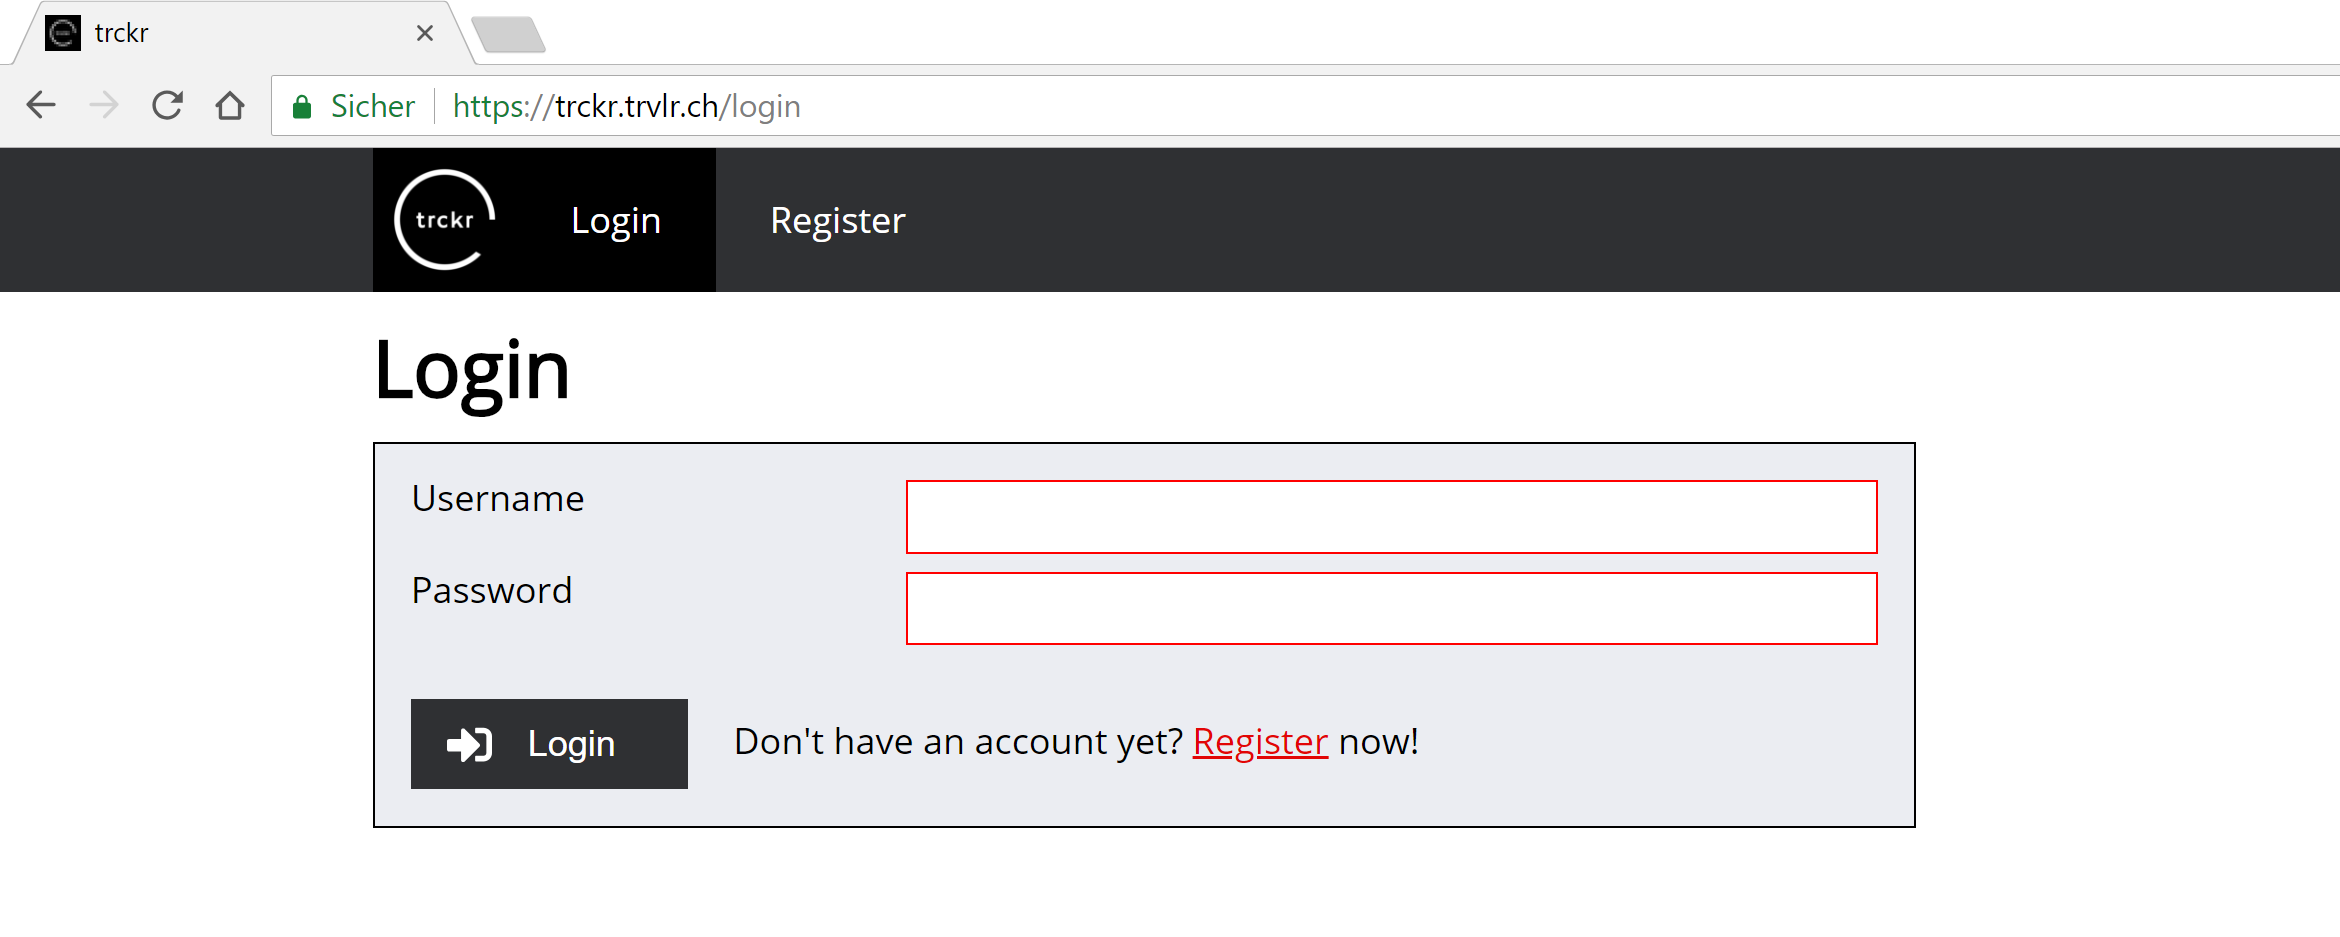
\includegraphics[width=\textwidth]{trckr-login}
    \caption{The trckr login page.}
    \label{fig:trckr-login}

    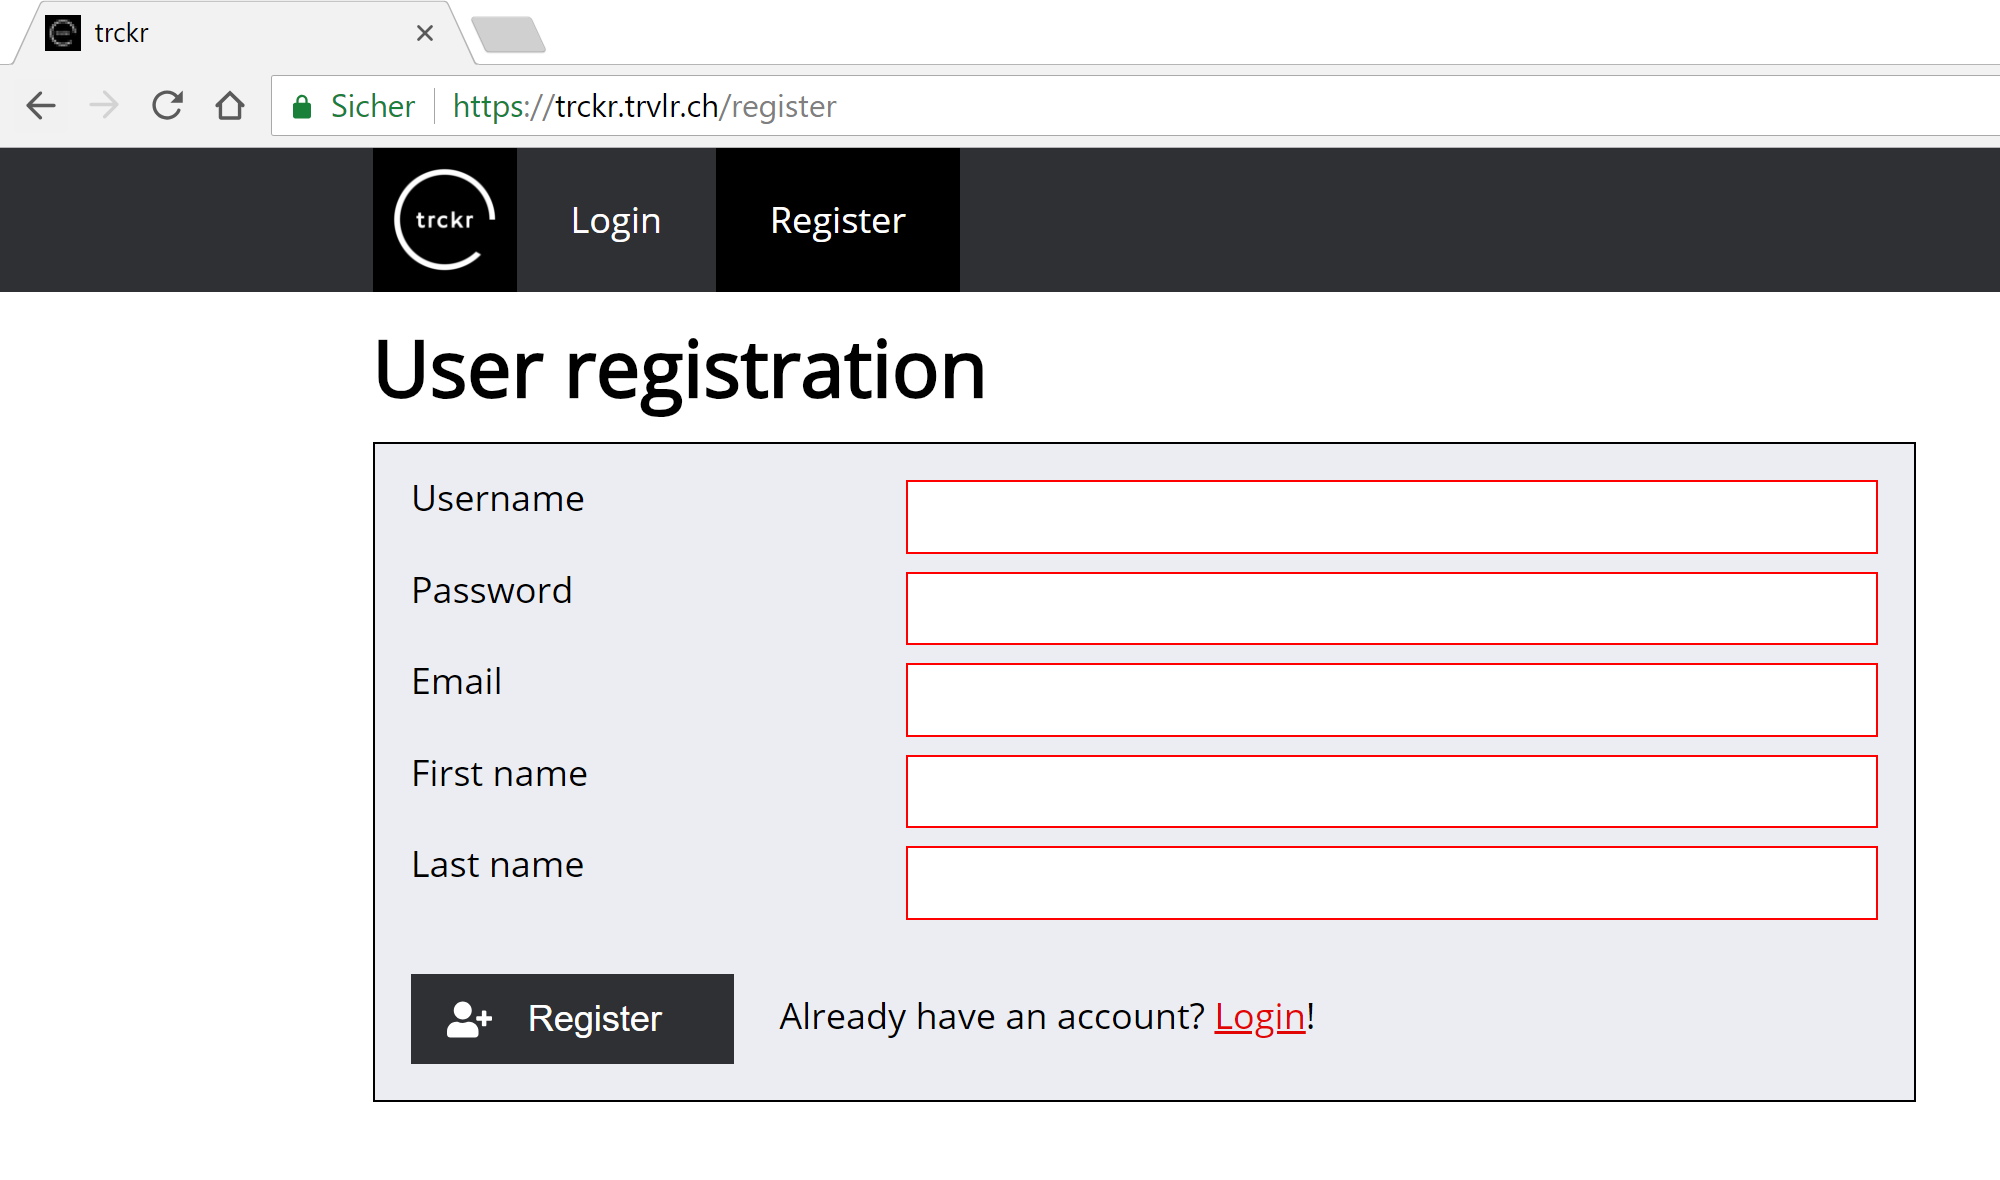
\includegraphics[width=\textwidth]{trckr-register}
    \caption{The trckr registration page.}
    \label{fig:trckr-register}
\end{figure}

The first thing one sees when visiting trckr, is that there is a login page.
For people that are not yet registered there is the option to register through a
"Register" link. Filling out the registration form will trigger a call to the
backend to create a user. The response to this call will contain an authentication
token, this allows the user to be logged in directly after registering.
Similarly, when submitting the login form the backend will reply with an
authentication token that allows an existing user to be logged in.\\
At the moment of registration the navigation bar on the top of the interface
will contain a link to the dashboard, the projects page, the time entries page
as well as a logout button.\\
The dashboard displays graphs...TODO \\

\begin{figure}[h]
    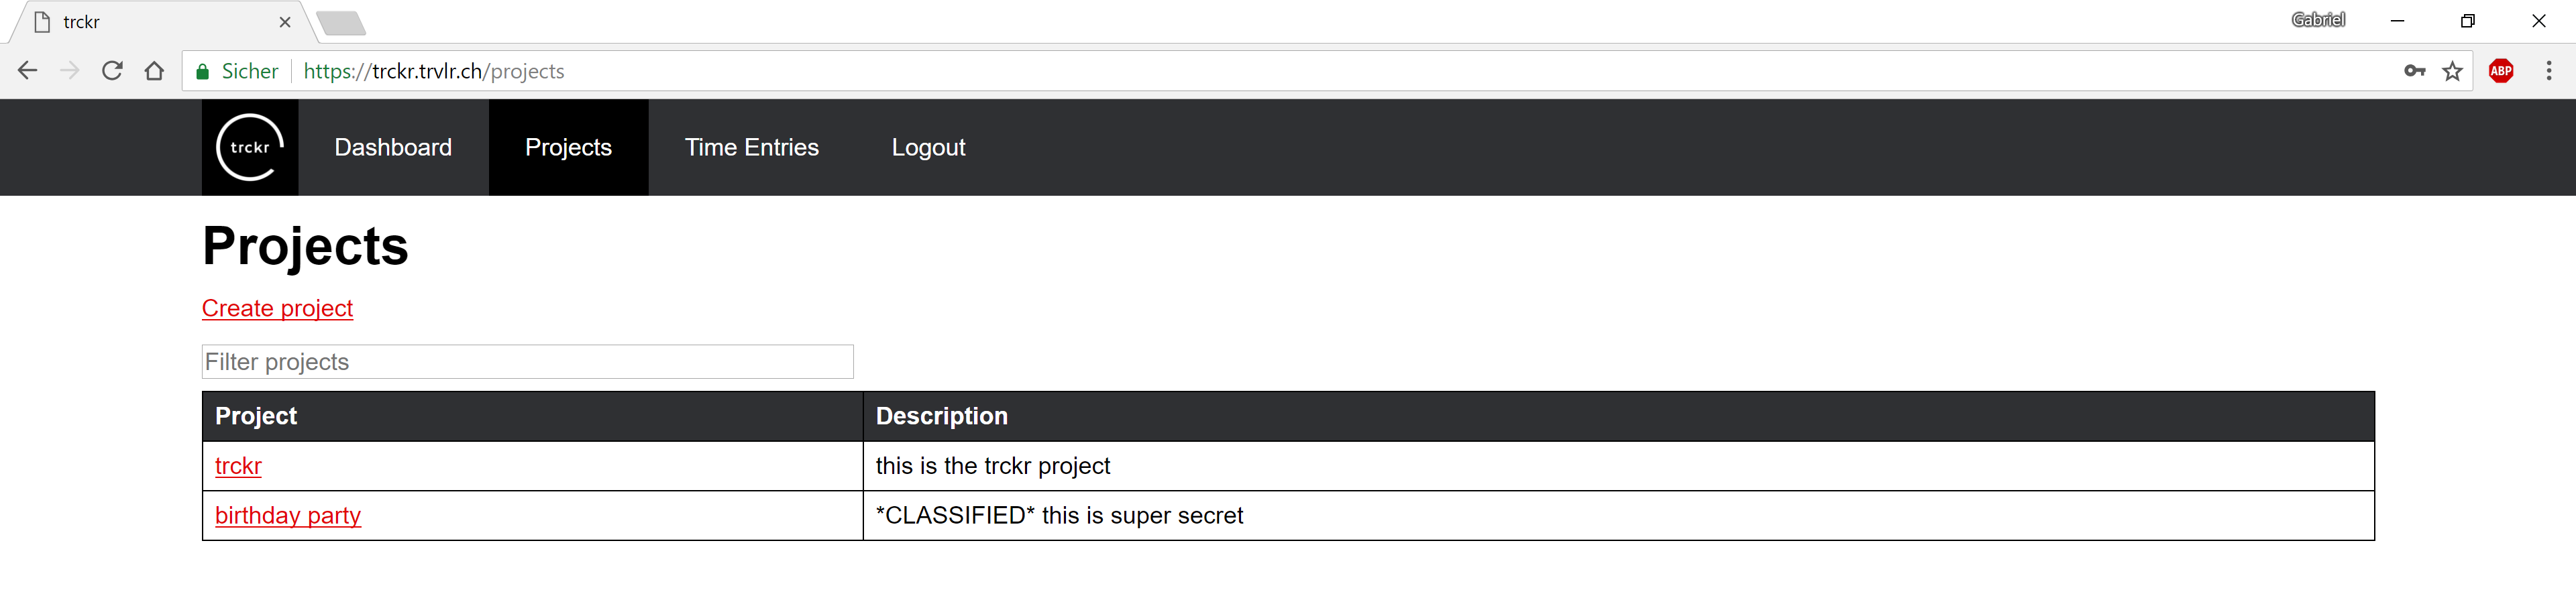
\includegraphics[width=\textwidth]{trckr-projects-table}
    \caption{The projects page.}
    \label{fig:trckr-projects-table}
\end{figure}

On the projects page one can see a table of all the projects that the currently
logged in user is a part of. The table is automatically generated by Vue.js and
it contains a row for each project. Above the projects table there is a
textfield that allows a user to filter for a project or a group of projects that
contain the given substring. To create a new project a user will have to
navigate to the projects page and click on the "Create project" link which will
open the project creation form. In this form a user can specify a name for the
project as well as an optional description.\\
Each project can be viewed in more detail when the project inside the table is
clicked. As the figure below is showing, the project page will contain the name,
the description and a table of all the tasks in the current project.

\begin{figure}[h]
    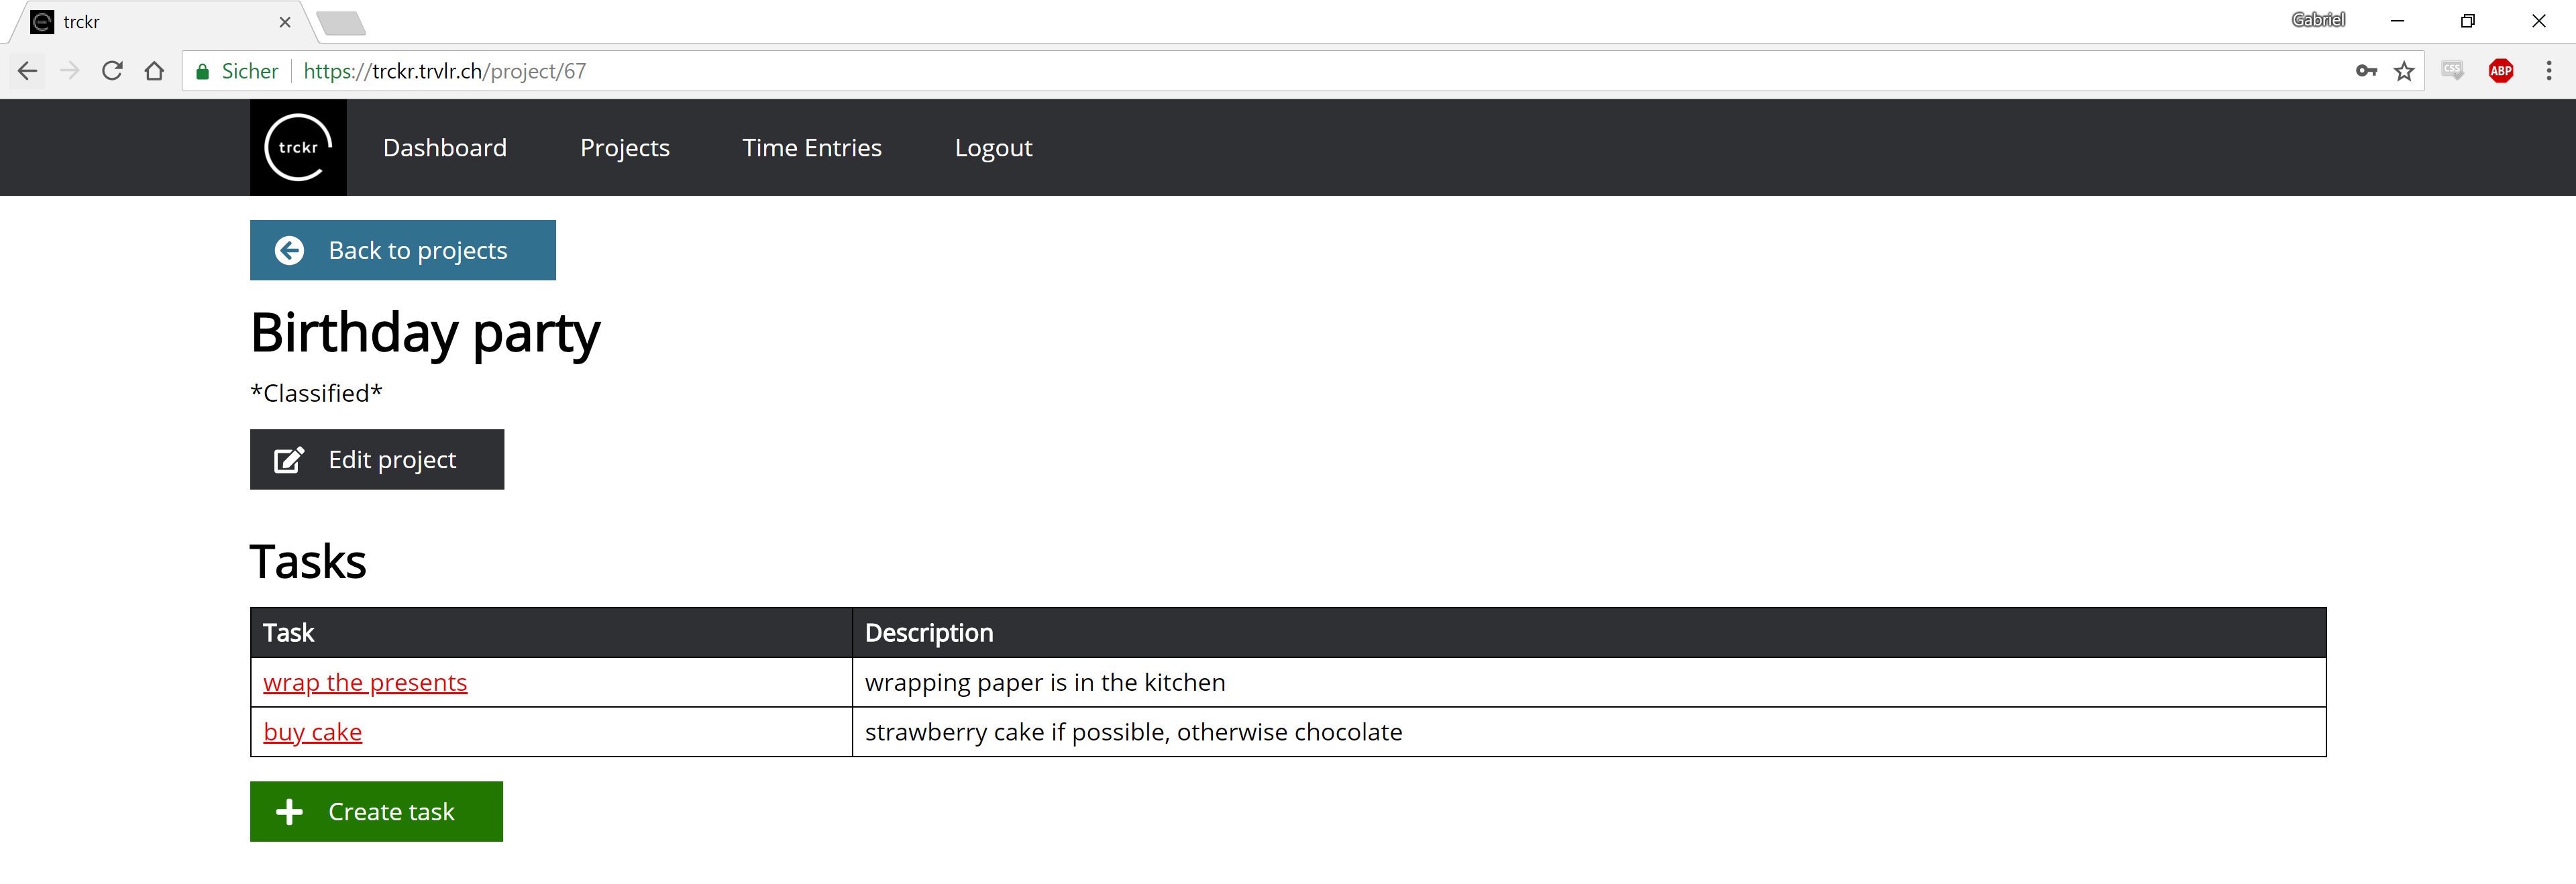
\includegraphics[width=\textwidth]{trckr-project-page}
    \caption{The projects page with the table of all projects.}
    \label{fig:trckr-project-page}
\end{figure}

Clicking on a task will display the details of said task, at the current state
that is only the name and the description of the task.\\
On the "Time Entries" page a user can create a time entry for a specific task of
a project. There is a link on the page that leads to the time entry form. In
said form the user has to choose a project first and then a task of the project
for which the time entry should be created.

\begin{figure}[h]
    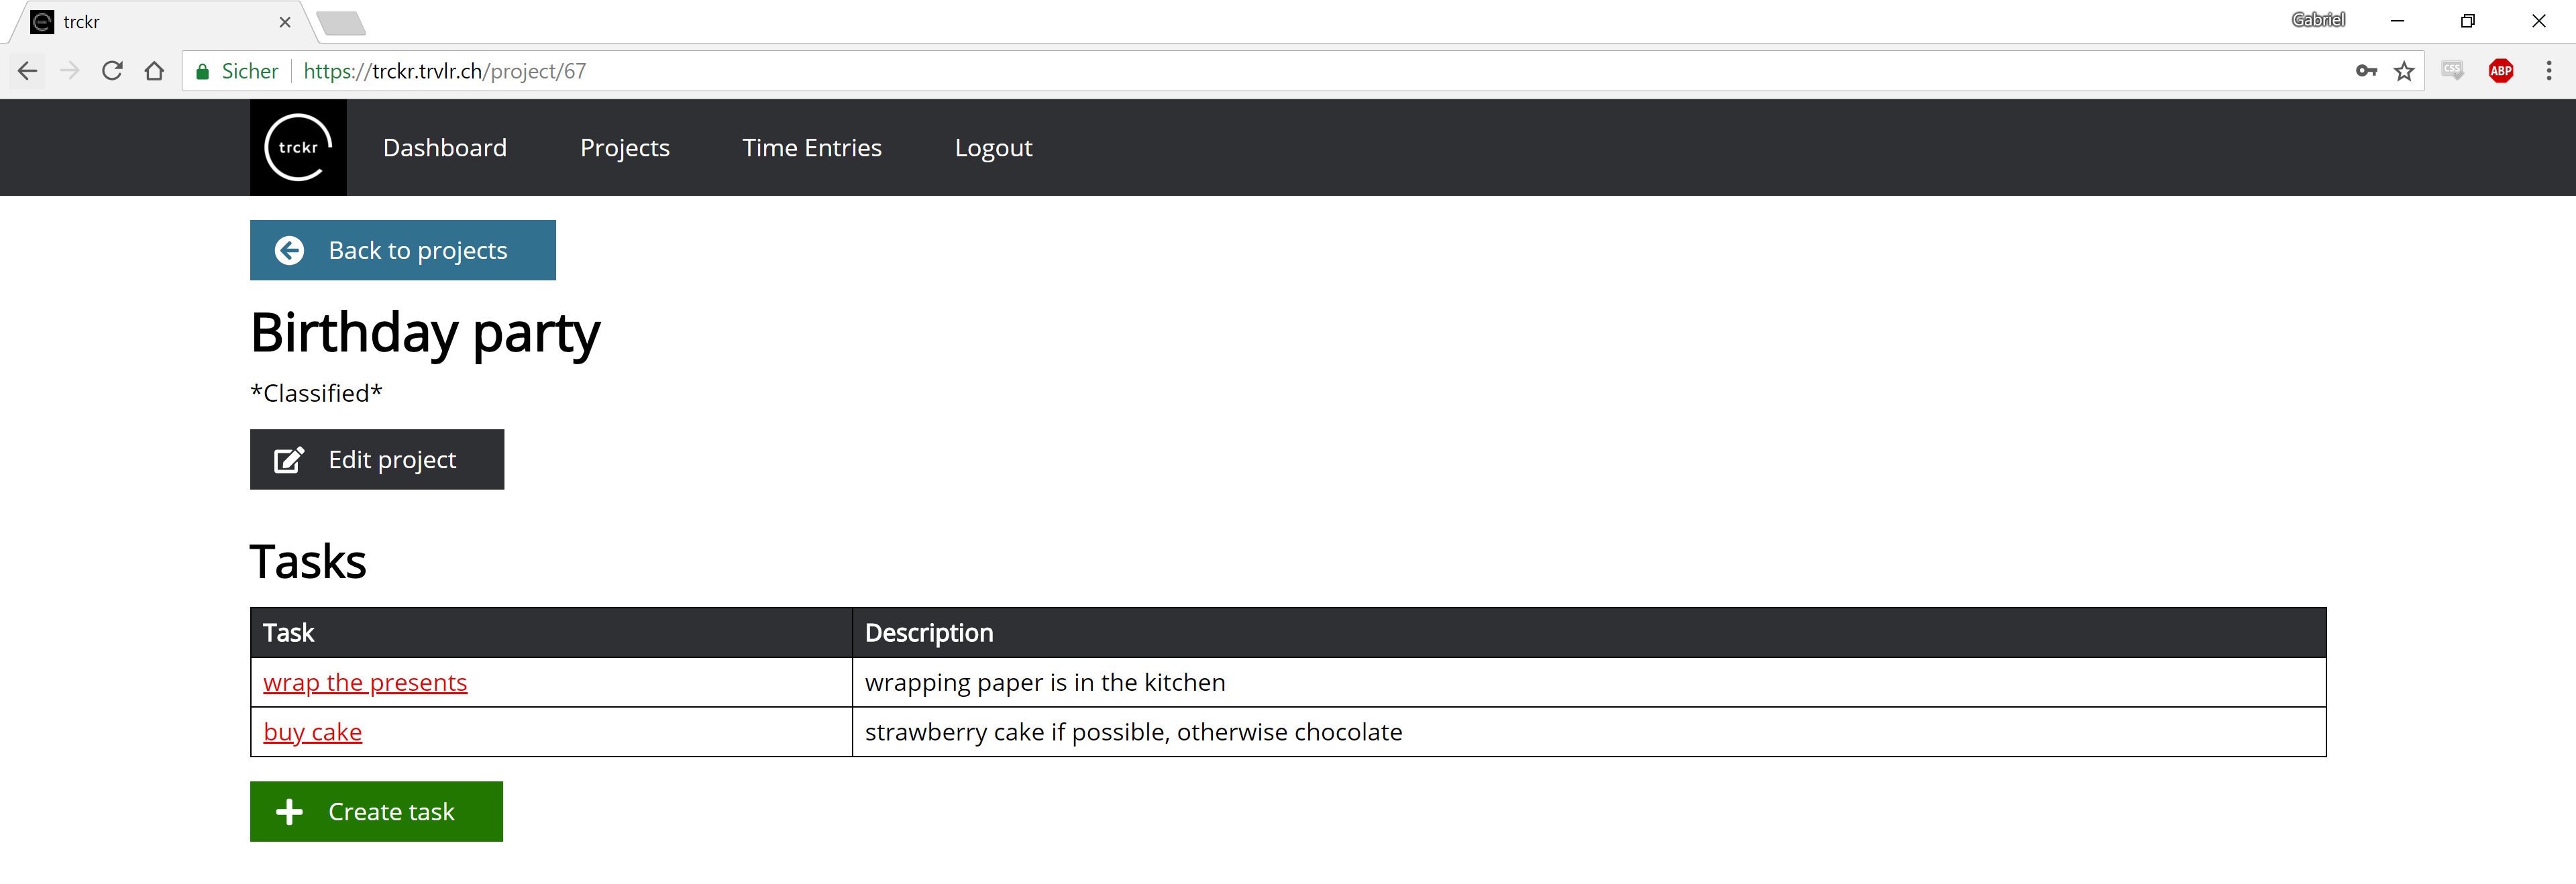
\includegraphics[width=\textwidth]{trckr-project-page}
    \caption{The form to add a time entry to a task.}
    \label{fig:trckr-create-time-entry}
\end{figure}

All time entries will be displayed on the time entry page.

% Outlook----------------------------------------------------------------------------
%   These are the informations printed on the title page of the article
% -------------------------------------------------------------------------------------------
\section{Outlook}
Outlook...

% Conclusion-----------------------------------------------------------------------------
%   These are the informations printed on the title page of the article
% -------------------------------------------------------------------------------------------
\section{Conclusion}
Conclusion...

% Bibliography-----------------------------------------------------------------------------
%   These are the informations printed on the title page of the article
% -------------------------------------------------------------------------------------------
\section{Bibliography}
Bibliography...
\begin{thebibliography}{9}

    \bibitem{vuejs}
    https://vuejs.org/ ; as 10.05.2018


\end{thebibliography}

\listoffigures

\end{document}
